\documentclass[hyperref={pdfpagelabels=false}]{beamer} %weil ist blöde und kann pdfpagelabels im beamer nicht aber versucht es trotzdem
\usepackage[utf8x]{inputenc} %soll utf8 als code verwenden
\PrerenderUnicode{äöüÄÖÜß} % umlaute gehen nun auch

\usepackage[ngerman]{babel} % deutsche Bezeichnungen

\usepackage{amsmath} % mathe formeln
\usepackage{amsthm} % mathe theoreme
\usepackage{graphicx} % Darstellung von Bildern

% - Times, Helvetica, Courier (Word Standard...)
\usepackage{mathptmx}
\usepackage[scaled=.90]{helvet}
\usepackage{courier}

\usepackage{beamerthemesplit} % das theme

% neue Theorem Blöcke
\newtheorem{thm}{Theorem}
\newtheorem{defin}{Definition}
\newtheorem{lem}{Lemma}
\newtheorem{beh}{Behauptung}

\title{Monotone vs. Non-monotone Circuit Complexity}
\author{Johannes Honke, Marko Jahn, Stephan Mielke}
\institute{BTU-Cottbus}
\date{23.09.2010}

\begin{document}

  \begin{frame}[plain]
    \titlepage
    \tableofcontents
  \end{frame}

  \section{Einführung: Funktionen}
  \begin{frame} %Stephan
    \frametitle{boolesche Funktionen}
    Eine Funktion ist eine Abbildung von einer Menge A in eine Menge B.\\
    In unserem Fall:
    $f: \{0,1\}^{n} \rightarrow \{0,1\}$ \\
    Also für jedes Tupel von Elementen am Eingang gibt es genau ein Element am Ausgang, das es repräsentiert.
  \end{frame}

  \section{Monotonie von Funktionen}
  \subsection*{Definition}
  \begin{frame}%Stephan
    \frametitle{Definition von Monotonie}
    Monotonie ist eine Eigenschaft von Funktionen.\\
    $f:A \rightarrow B: \forall x_1,x_2 \in A : (x_1 \leq_A x_2 \Rightarrow f(x_1) \leq_B f(x_2))$\\
    Um die Mengen ordnen zu können, brauchen wir Ordnungsrelationen.\\
    Wir benutzen hier die Ordnungsrelation $\leq_A$ für die Menge A\\
    und $\leq_B$ für die Menge B.\\
  \end{frame}

  \subsection*{Allgemeine Beispiele}
  \begin{frame}
    \frametitle{Monotonie Beispiele}
    Allgemeine Beispiele für monotone Funktionen:\\
    \begin{tabular}[t]{ll}
      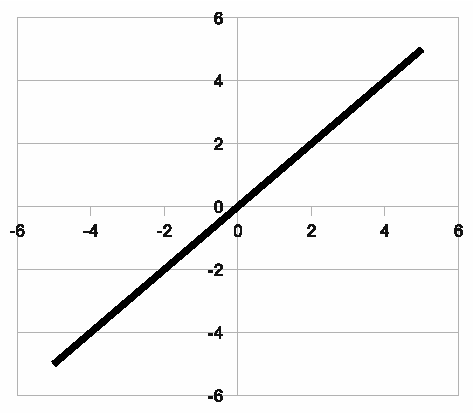
\includegraphics[scale=0.35]{images/f1.pdf} & $f(x) = m * x + n$
    \end{tabular}
    \\Beispiele für NICHT monotone Funktionen:\\
    \begin{tabular}[t]{ll}
      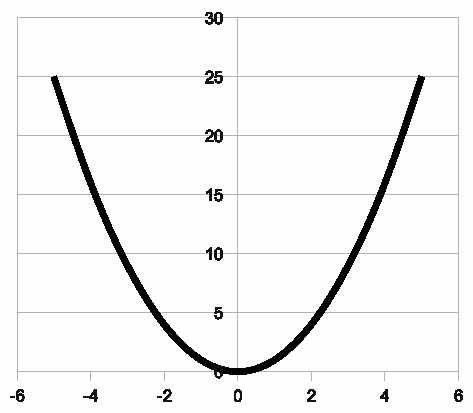
\includegraphics[scale=0.35]{images/f2.pdf} & $f(x) = a * x^2 + b * x + c$
    \end{tabular}
  \end{frame}

  \subsection{Ordnungsfunktionen}
  \begin{frame}%Stephan
    \frametitle{Ordnungfunktionen}
    Monotonien bilden eine partielle Ordnung.\\ Es sind also folgende Eigenschaften erfüllt:\\
    \begin{itemize}
      \item reflexiv $\forall a \in A: (a,a) \in B$\\
      \item transitiv $\forall a,b,c \in A: (a,b) \in B \land (b,c) \in B \Rightarrow (a,c) \in B$\\
      \item antisymmetrisch $\forall a,b \in A: (a,b) \in B \land (b,a) \in B \Rightarrow a=b$\\
    \end{itemize}
    Es ergeben sich also folgende monotone Grundgatter:\\
    \begin{tabular}[t]{|cc|c|c|c|c|c|c|} \hline
      $x_1$	& $x_2$	& AND	& OR	& 0	& 1	& $p_1$	& $p_2$\\ \hline
      0	& 0	& 0	& 0	& 0	& 1	& 0	& 0\\
      0	& 1	& 0	& 1	& 0	& 1	& 0	& 1\\
      1	& 0	& 0	& 1	& 0	& 1	& 1	& 0\\
      1	& 1	& 1	& 1	& 0	& 1	& 1	& 1\\ \hline
    \end{tabular}
  \end{frame}

  \subsection{Ordnungsrelations-Beispiele}
  \subsubsection*{Ordnungsrelation Beispiel mit Tupel n = 1}
  \begin{frame}
    \begin{figure}
      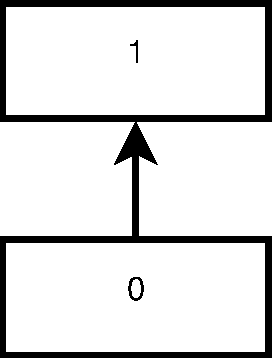
\includegraphics[scale=0.30]{images/m1.pdf}
      \caption{Anstieg des Tupels n = 1}
      Die Ordnungsrelation ist einfach ablesbar.
    \end{figure}
  \end{frame}

  \subsubsection*{Ordnungsrelation Beispiel mit Tupel n = 2}
  \begin{frame}
    \begin{figure}
      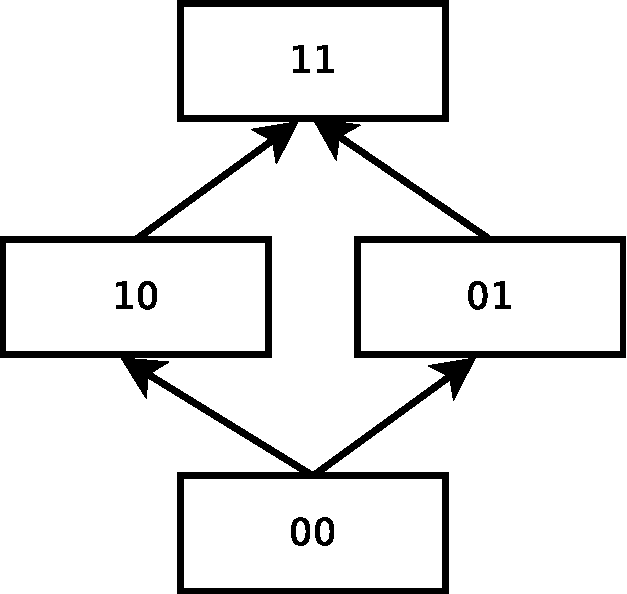
\includegraphics[scale=0.30]{images/m2.pdf}
      \caption{Anstieg des Tupels n = 2}
      Die Ordnungsrelation ist einfach ablesbar.
    \end{figure}
  \end{frame}

  \subsubsection*{Ordnungsrelation Beispiel mit Tupel n = 3}
  \begin{frame}
    \begin{figure}
      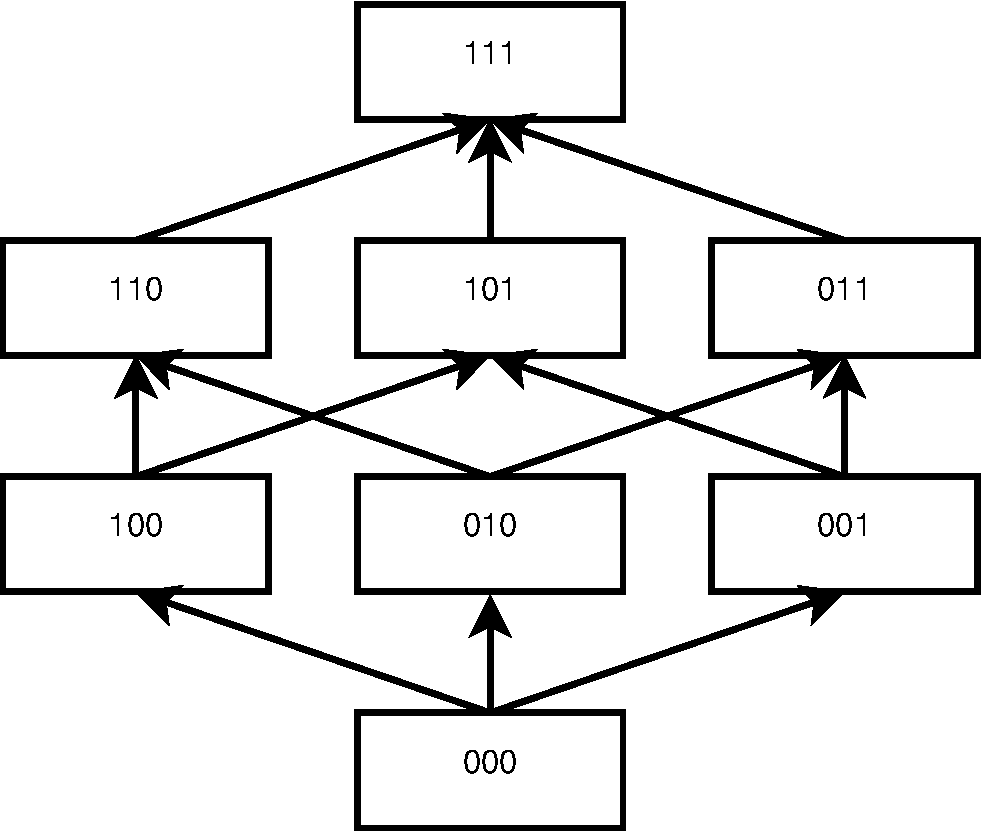
\includegraphics[scale=0.30]{images/m3.pdf}
      \caption{Anstieg des Tupels n = 3}
      Die Ordnungsrelation ist NICHT mehr einfach ablesbar.
    \end{figure}
  \end{frame}

  \subsubsection*{Ordnungsrelation Beispiel mit Tupel n = 4}
  \begin{frame}
    \begin{figure}
      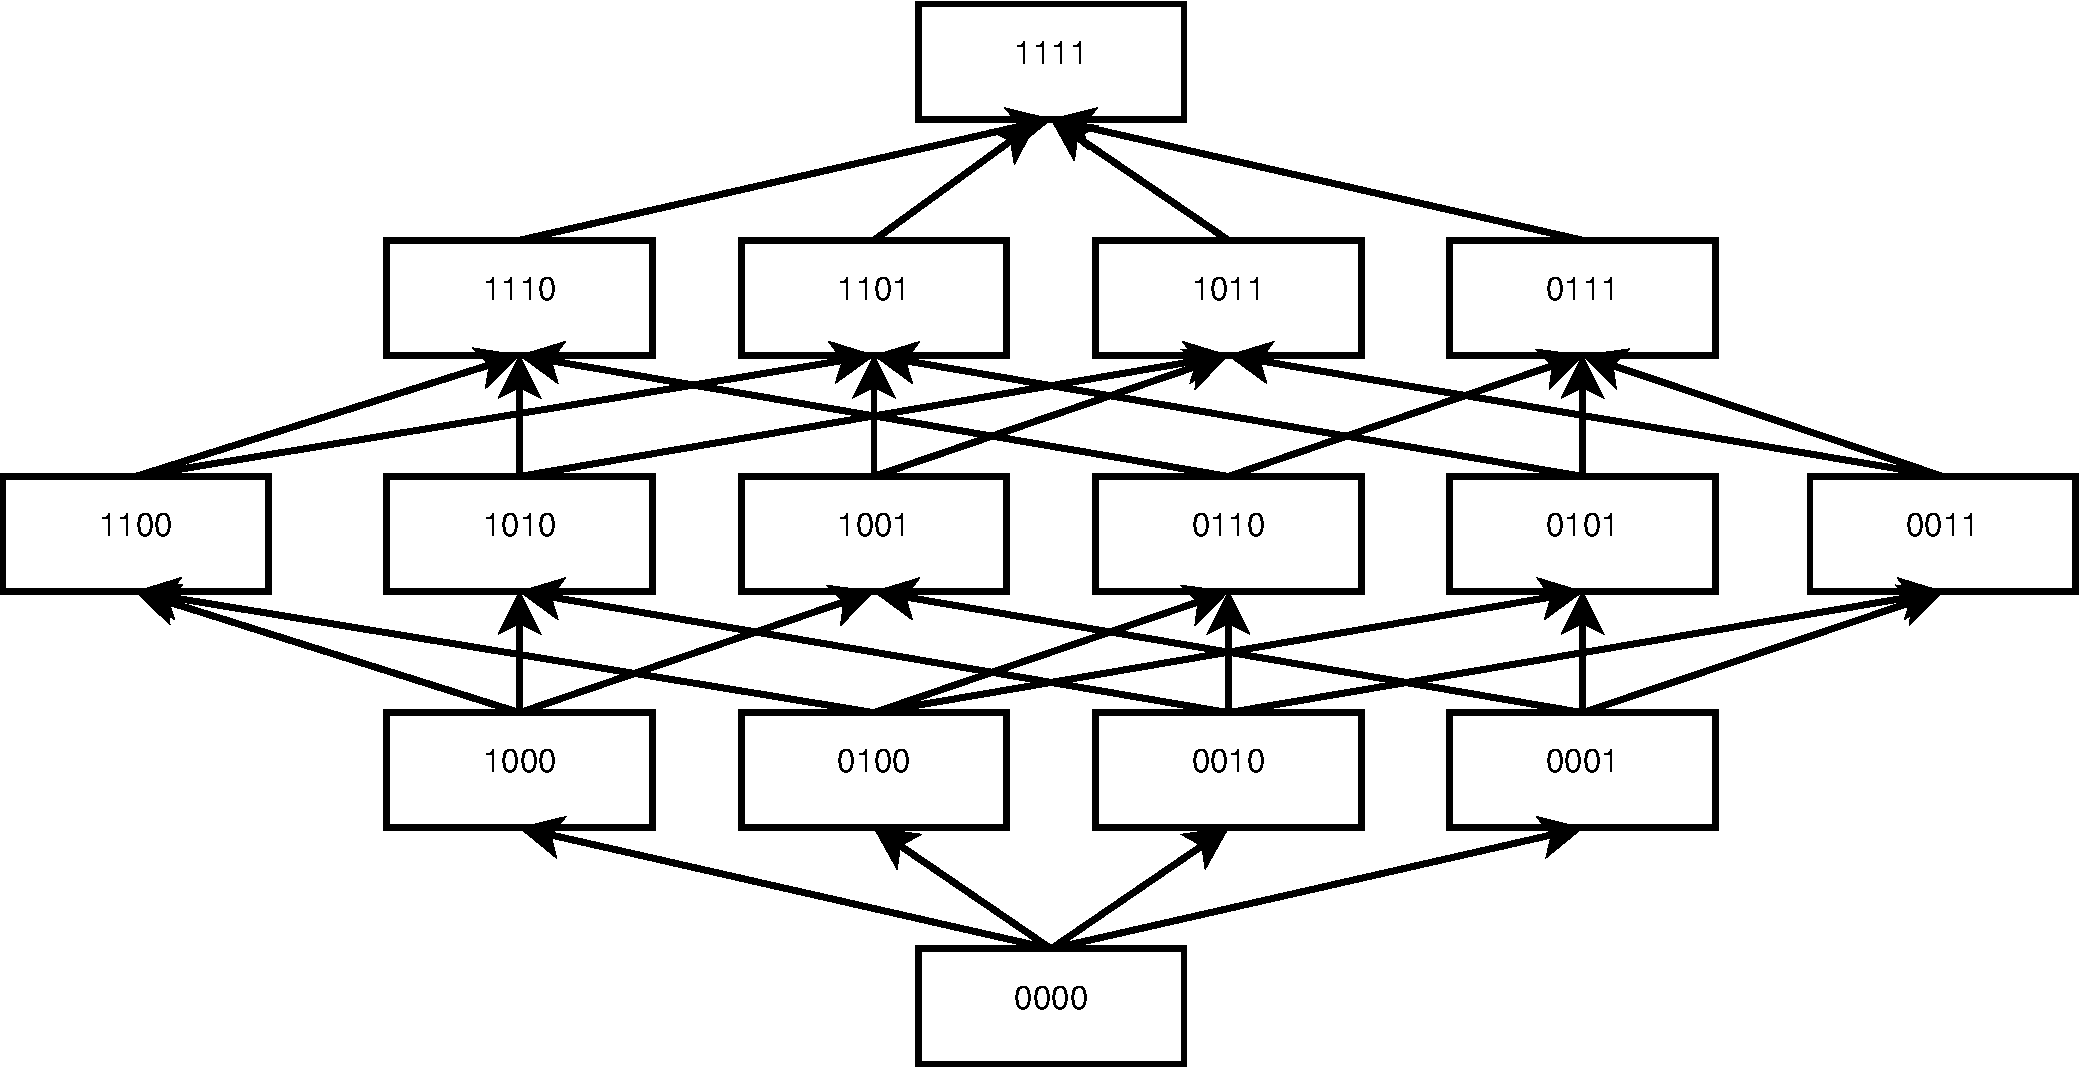
\includegraphics[scale=0.30]{images/m4.pdf}
      \caption{Anstieg des Tupels n = 4}
      Die Ordnungsrelation ist kompliziert.
    \end{figure}
  \end{frame}

  \section{Komplexität}
  \subsection*{in Worten}
    \begin{frame}%Johanes
    \frametitle{Komplexität in Worten}
    Die Komplexität ist ein Maß für den Aufwand einer Funktion.
    Hierbei geht es um den Verbrauch von Ressourcen, die Größe (Anzahl der Gatter) sowie die Tiefe (längster Pfad)
    eines Schaltkreises.\\
  \end{frame}

  \subsection*{in Formeln}
  \begin{frame}
    \frametitle{Komplexität in Formeln}
    \begin{itemize}
      \item $C(f) = min \{G(S(f))\}$
      \item $S(f)$ "best" möglichen SK für die Funktion $f(x)$
      \item $C_M(f) = min \{G(S_M(f))\}$
      \item $S_M(f)$ "best" möglichen monotonen SK für die Funktion $f(x)$
      \item $G(S)$ Anzahl der Gatter der Funktion $f(x)$, also die Größe
    \end{itemize}
  \end{frame}

  \subsection{Theorem von Tardos}
  \begin{frame}
    \frametitle{Theorem von Tardos}
    Für den Unterschied zwischen einem monotonen und einem nicht monotonen Schaltkreis in Bezug auf die Größe gilt, das seine nicht monotone Variante die untere Schranke für den monotonen bildet.
    \begin{thm}[Tardos]
      Die Lücke zwischen $C_{M}$ und $C$ ist exponentiell.
    \end{thm}
    Das heißt also: Je größer ein Schaltkreis ist, umso größer ist der Abstand der Komplexit\"aten, der monotonen Lösung von der nicht-monotonen.\\
    $\forall f(x)_n, f(x)_{n+1} \in \{0,1\}:$\\$(C_M(f(x)_n) - C(f(x)_n)) \leq (C_M(f(x)_{n+1}) - C(f(x)_{n+1})$
  \end{frame}

  \section{Slice-Funktionen}
  \subsection*{Definition}
  \begin{frame}%Marko
    \frametitle{Definition von Slice-Funktionen}
    \begin{defin}
      Eine Funktion $f:\{0,1\}^n \rightarrow \{0,1\}$ hat Slice(Teil)-Funktionen, wenn glit:\\

      $\sum_{i=1}^{n} x_i<k\Rightarrow f(x)=0$\\

      $\sum_{i=1}^{n} x_i>k\Rightarrow f(x)=1$\\
    \end{defin}
    Eine boolesche Funktion hat mehrere Slice(Teil)-Funktionen, wenn der Ausgang der Funktion $1$ ist obwohl nicht alle Eingangswerte $1$ sein mussten.
    Das $k \in \mathbb{N}$ gibt die Anzahl an wie viele Eing\"ange auf $1$ sein mussten.
    Somit kann man die Funktion teilen in kleinere Funktionen die nicht mehr alle Eing\"ange haben aber immer noch f\"ur die noch existieren logisch \"aquivalent zur Mutter-Funktion sind.
  \end{frame}

  \subsection*{die Monotonie}
  \begin{frame}
    \frametitle{Monotonie von Slice-Funktionen}
    Für eine gegebene Funktion $f:\{0,1\}^n \rightarrow \{0,1\}$ können wir den k-ten Slice von $f$,
    $f^{(k)}$ wie folgt definieren:\\
    \begin{defin}
      \begin{align*}
        f^{(k)}(x) =
        \begin{cases}
          0 & \sum\nolimits_{i=1}^{n} x_i < k\\
          1 & \sum\nolimits_{i=1}^{n} x_1 > k\\
          f(x) &\sum\nolimits_{i_1}^{n} x_i = k
        \end{cases}
      \end{align*}
    \end{defin}
    Beobachtung: Slice-Funktionen sind monoton.\\
    Da für alle $Elemente < k$ eine $0$ steht und für alle $> k$ eine $1$, ist somit der Umschlag von $0$ auf $1$ bei oder nach dem $k$.
  \end{frame}

  \subsection{im Schaltkreis}
  \begin{frame}%Johanes
    \frametitle{Slice-Funktionen im Schaltkreis}
    \begin{lem}
      Für jeden $U_2$ Schaltkreis $\beta$ gibt es einen äquivalenten Schaltkreis, welcher höchstens
      2 mal so groß ist wie $\beta$, bei dem nur NOT-Gatter bei den Variablen benutzt werden. %9.4 Johanes
    \end{lem}
    Es wird der jeweilige Schaltkreis erweitert, wobei jedes nicht-monotone Gatter in monotone Grundgatter zerlegt wird und die NOT-Gatter werden von innen nach außen, bis zur Variablen / Input Ebene, verschoben werden.
    \\Beweis durch Konstruktion.
  \end{frame}

  \subsection{die Komplexität}
  \begin{frame}%Stephan
    \frametitle{die Komplexität von Slice-Funktionen}
    \begin{beh}
      $C(f) \leq C(f^{(0)}, f^{(1)}, \dots ,f^{(n)})+h(n)$\\
    \end{beh}
    \begin{itemize}
      \item $C(f^{(0)}, f^{(1)}, \dots ,f^{(n)})$ ist die Gesamtkomplexität für den SK, der alle Slice-Funktionen $f(x)^{(n)}$ von $f(x)$ beinhaltet
      \item $h(n) \in \mathbb{N}$ die benötigte Komplexität für den Multiplexer, der das Ergebnis zuweist
      \item $h \in \mathcal{O}(n)$
      \item $n$ Anzahl der Eingänge
    \end{itemize}
  \end{frame}

  \subsubsection*{Vorteile}
  \begin{frame}
    \frametitle{Vorteile von Slice-Funktionen}
    \begin{beh}
      $C(f^{(0)}, f^{(1)}, \dots f^{(n)}) \leq \sum_{i=0}^{n}{C(f^{(i)})}$ für das ein $k \in \{1, \dots n\}$\\
      existiert in $C(f^{(k)}) \geq \frac{C(f)}{n} - h(1)$
    \end{beh}
    \begin{itemize}
      \item wie schon gesagt: $f(x)$ wird für alle auftretenen Fälle gleichzeitig berechnet
      \item der Multiplexer ist an die Eingänge der Funktion gekoppelt
      \item er wählt so den richtigen Ausgang der Funktion und schaltet ihn durch
    \end{itemize}
  \end{frame}

  \subsection*{Grenzen der Komplexität}
  \begin{frame}%Marko
    \frametitle{Grenzen der Komplexität von Slice-Funktionen}
    \begin{thm}
      Wenn $f$ eine Slice-Funktion ist, dann gilt:
      $C(f) \leq C_M(f) \leq (C(f) +n^2 log\;n)$%9.5 Marko
    \end{thm}
    Die Komplexität der monotonen Variante einer Funktion ist bis zu $n^2 log\;n$ größer als die geringste Komplexität seiner nicht monotonen.\\
    Also ist die $C(f)$ die untere und $C(f) + n^2 log\;n$ die obere Schranke für $C_M(f)$.
  \end{frame}

  \section{Abschließende Fragen}
  \begin{frame}%Marko
    \frametitle{Randolfs Fragen}
    \begin{block}{Gibt es für jede monotone Funktion einen monotonen Schaltkreis?}
      Ja, die DNF besteht zwar aus NOT-Gattern, jedoch, wenn die Funktion monoton war, bleibt die Funktion bestehen, wenn man alle verneinten Variablen entfernt.
    \end{block}
    \begin{block}{Berechnet jeder monotone Schaltkreis eine monotone Funktion?}
      Ja, da der Schaltkreis nur aus monotonen Grundgattern (AND, OR, 0, 1 und die Projektionen) bestehen darf, ist die daraus folgende Funktion auch immer monoton.
    \end{block}
  \end{frame}

  \section{Zusammenfassung}
  \begin{frame}
    \frametitle{behandelte Themen}
    \begin{itemize}
      \item Monotonie
      \item Komplexität
      \item Slice-Funktionen
      \begin{itemize}
        \item im Schaltkreis
        \item Komplexität
        \item Grenzen der Komplexität
      \end{itemize}
    \end{itemize}
  \end{frame}

\end{document}